% !TEX program = lualatex
% Compile from 2026/week1: latexmk -lualatex slide.tex
% Source: ../../2025/week1/slide.pptx (14 slides, 4:3).
% Dates follow the 2026 university calendar.
\documentclass[12pt,aspectratio=43]{beamer}
% Shared Beamer design. Load after \documentclass using \input.
% Engine: LuaLaTeX. Fonts: UD Digi Kyokasho N (regular/bold), Arial.
\usepackage{luatexja-fontspec}
\setmainjfont[BoldFont={UD Digi Kyokasho N Bold}]{UD Digi Kyokasho N}
\setsansjfont[BoldFont={UD Digi Kyokasho N Bold}]{UD Digi Kyokasho N}
\setmonojfont[BoldFont={UD Digi Kyokasho N Bold}]{UD Digi Kyokasho N}
\setmainfont{Arial}
\setsansfont{Arial}
\setmonofont{Arial}
\renewcommand{\kanjifamilydefault}{\gtdefault}

% Typeset mathematics with a dedicated TeX math font, independent of Arial.
\usefonttheme{professionalfonts}
\usepackage[mathrm=sym]{unicode-math}
\setmathfont{Latin Modern Math}
\setoperatorfont{\symup}

\definecolor{courseblue}{HTML}{4472C4}
\definecolor{ruleblue}{HTML}{8FAADC}
\setbeamercolor{normal text}{fg=black,bg=white}
\setbeamercolor{structure}{fg=courseblue}
\setbeamercolor{frametitle}{fg=black,bg=white}
\setbeamercolor{title banner}{fg=white,bg=courseblue}
\setbeamerfont{frametitle}{size=\fontsize{18}{22}\selectfont,series=\mdseries}
\setbeamerfont{quote}{shape=\upshape}
\setbeamersize{text margin left=9mm,text margin right=9mm}
\setbeamertemplate{navigation symbols}{}
\setbeamercolor{page number}{fg=gray,bg=white}
\setbeamertemplate{footline}{%
  \begin{beamercolorbox}[wd=\paperwidth,ht=2.5mm,dp=1.5mm]{page number}
    \hfill{\fontsize{8}{9}\selectfont
      \ifnum\value{framenumber}>0
        \insertframenumber\,/\,\inserttotalframenumber
      \fi}\hspace*{3mm}
  \end{beamercolorbox}}
\setbeamertemplate{headline}{%
  \hfill\textcolor{gray}{\fontsize{6}{7}\selectfont
    \hypersetup{linkcolor=gray}% Keep Beamer's title links in the header color.
    \ifnum\value{framenumber}=0 \insertshortdate\enspace\fi
    \insertshorttitle\space\insertshortsubtitle}\hspace{2mm}\vspace{1.5mm}}
\setbeamertemplate{frametitle}{%
  \vspace{2mm}\centering\insertframetitle\par
  \vspace{-1mm}{\color{ruleblue}\rule{.44\paperwidth}{.5pt}}\par
  \vspace{2mm}}
\setbeamercolor{itemize item}{fg=courseblue}
\setbeamercolor{itemize subitem}{fg=black}
\setbeamercolor{itemize subsubitem}{fg=black}
\setbeamertemplate{itemize item}{\textbullet}
\setbeamertemplate{itemize subitem}{\textnormal{-}}
\setbeamertemplate{itemize subsubitem}{\textnormal{-}}
\setlength{\parskip}{.45em}
\hypersetup{colorlinks=true,urlcolor=courseblue}

% Use \titlepage inside a [t,noframenumbering] frame. The background extends
% 1 mm past both page edges to avoid hairline gaps in PDF viewers.
\setbeamertemplate{title page}{%
  \vspace{2mm}
  \begin{beamercolorbox}[wd=\paperwidth,ht=43mm,dp=13mm,colsep*=1mm,center]{title banner}
    {\fontsize{32}{40}\selectfont\inserttitle\par}
    \vspace{2mm}
    {\fontsize{20}{24}\selectfont\insertsubtitle\par}
  \end{beamercolorbox}
  \vspace{10mm}
  \hfill\insertauthor
}

\usepackage{graphicx}
\usepackage{array}
\usepackage{tikz}
\usetikzlibrary{arrows.meta}
\graphicspath{{slide-assets/}}
\newfontfamily\codefont{Consolas}
\definecolor{codevalue}{HTML}{7A3E9D}
\definecolor{codebuiltin}{HTML}{006DB0}
\definecolor{codestring}{HTML}{267348}
\newcommand{\playicon}{\tikz[baseline=-.3mm]{%
  \fill (0,0) -- (0,.24) -- (.21,.12) -- cycle;}}

% Editable notebook cells: execution number, two code lines, and output.
\newcommand{\pythonexample}[4]{%
  \begin{beamercolorbox}[wd=\linewidth,sep=1.8mm]{example code}
    {\codefont\fontsize{9}{10}\selectfont\textcolor{courseblue}{In [#1]:}\par}
    \begingroup\codefont\fontsize{16}{18}\selectfont
      \strut#2\\
      \strut#3\par
    \endgroup
  \end{beamercolorbox}\par
  \begin{beamercolorbox}[wd=\linewidth,sep=.5mm,leftskip=1.3mm]{example output}
    {\fontsize{9}{11}\selectfont\textcolor{black!65}{出力}}\quad
    {\codefont\fontsize{16}{18}\selectfont\strut#4}
  \end{beamercolorbox}}

% A single expression and its displayed notebook result.
\newcommand{\pythonresult}[3]{%
  \begin{beamercolorbox}[wd=\linewidth,sep=1.8mm]{example code}
    {\codefont\fontsize{9}{10}\selectfont\textcolor{courseblue}{In [#1]:}\par}
    {\codefont\fontsize{16}{18}\selectfont\strut#2\par}
  \end{beamercolorbox}\par
  \begin{beamercolorbox}[wd=\linewidth,sep=.5mm,leftskip=1.3mm]{example output}
    {\fontsize{9}{11}\selectfont\textcolor{black!65}{出力}}\quad
    {\codefont\fontsize{16}{18}\selectfont\strut#3}
  \end{beamercolorbox}}

\title{計算物理学B}
\subtitle{第一回}
\author{野垣 康介、藤本 悠輝}
\date{2026/10/06}
\hypersetup{pdftitle={計算物理学B 第一回},pdfauthor={野垣 康介、藤本 悠輝}}

% Coordinates for screenshot annotations run from (0,0) at the lower left
% to (1,1) at the upper right. Screenshots themselves remain original PNGs.
\newcommand{\screenshot}[3]{%
  \begin{tikzpicture}
    \node[anchor=south west,inner sep=0] (screen) at (0,0)
      {\includegraphics[width=#2]{#1}};
    \begin{scope}[x={(screen.south east)},y={(screen.north west)}]
      #3
    \end{scope}
  \end{tikzpicture}}

\begin{document}

% 1 -------------------------------------------------------------------
\begin{frame}[t,noframenumbering]
  \titlepage
\end{frame}

% 2 -------------------------------------------------------------------
\begin{frame}{はじめに}
  \begin{itemize}
    \setlength{\itemsep}{3mm}
    \item 本講義は火曜3限の「計算物理学B」です
    \item 講義室はB201です。
      \begin{itemize}
        \item 講義室のコンセントは限られているため、PCを十分に充電した状態で授業に臨んでください。
      \end{itemize}
    \item 毎回の講義は、前半の座学と後半の実習に分かれています。
    \item 成績評価について
      \begin{itemize}
        \setlength{\itemsep}{1mm}
        \item 中間・期末2回のレポート（100\%）
        \item 毎回の出席点は、救済措置とします。
        \item 出席点は、授業中の成果物で評価
      \end{itemize}
  \end{itemize}
\end{frame}

% 3 -------------------------------------------------------------------
\begin{frame}{自己紹介}
  \begingroup\fontsize{14}{17}\selectfont 野垣 康介\par\endgroup
  \par\begingroup\small\leftskip=5mm\relax\parskip=0pt
    専門は、物性理論\\
    C/C++、Fortran90、Julia、Pythonがわかります\\
    授業はPythonですが、その他の言語の質問もわかる範囲で答えます\\
    スパコンを用いた大規模シミュレーションを得意としています
  \par\endgroup
  \begingroup\fontsize{14}{17}\selectfont 藤本 悠輝（育休中）\par\endgroup
  \par\begingroup\small\leftskip=5mm\relax\parskip=0pt
    専門は原子核理論（クォーク・ハドロン物理学）\\
    主にPythonを使用するほか、C/C++とMathematicaもわかります\\
    研究では、解析計算とラップトップで動く程度の数値計算とを組合せています\\
    機械学習の応用の経験があります
  \par\endgroup
\end{frame}

% 4 -------------------------------------------------------------------
% Calendar: https://www.niigata-u.ac.jp/wp-content/uploads/2025/08/schedule_2026.pdf
% 10/13 follows Monday's timetable; 11/6 follows Tuesday's timetable.
% Cancel 10/20 for travel; teach on 12/1; no makeup on 2/9.
% Exclude 11/3 and winter recess (12/27--1/6). Updated 2026/10/05.
% Topics follow the lecture schedule on page 2 of ../../2025/week14/week14.pdf.
\begin{frame}{講義予定}
  2026年度 第2学期（火曜3限）
  \par
  {\centering
    \renewcommand{\arraystretch}{1.05}
    \begin{tabular}{@{}l@{\hspace{2mm}}l@{\hspace{4mm}}l@{\hspace{2mm}}l@{}}
      10/6 & 四則演算 & 12/8 & モンテカルロ1 \\
      10/27 & 制御文（for, if） & 12/15 & モンテカルロ2 \\
      \textcolor{courseblue}{11/6 (金)} & 関数 & 12/22 & 微分方程式1 \\
      11/10 & 配列（numpy） & 1/12 & 微分方程式2 \\
      11/17 & 可視化（matplotlib） & 1/19 & 偏微分方程式1 \\
      11/24 & 数値微分 & 1/26 & 偏微分方程式2 \\
      12/1 & 数値積分 & 2/2 & 根の探索
    \end{tabular}
    \par}
  \begingroup\small
    \textcolor{courseblue}{10/20は出張で休講。}\\
    11/6（金）は火曜日授業の振替日。\\
    あくまで予定なので変更の可能性あり
  \par\endgroup
  {\fontsize{7}{8}\selectfont
    日付：\href{https://www.niigata-u.ac.jp/wp-content/uploads/2025/08/schedule_2026.pdf}{令和8年度（2026）新潟大学授業暦}\par}
\end{frame}

% 5 -------------------------------------------------------------------
\begin{frame}{実習環境}
  \begin{itemize}
    \setlength{\itemsep}{6mm}
    \item プログラミング環境は、Google Colab上のPython環境を推奨します。
      \begin{itemize}
        \setlength{\itemsep}{1mm}
        \item 授業で公式にサポートする環境です。
        \item \url{https://colab.research.google.com/?hl=ja}
      \end{itemize}
    \item プログラミング経験のある人は、ローカルの環境を使用しても構いません。
      \begin{itemize}
        \item 課題提出の際は、仮想環境の\texttt{requirements.txt}を一緒に提出してください。
      \end{itemize}
  \end{itemize}
\end{frame}

% 6 -------------------------------------------------------------------
\begin{frame}[t]{Google Colab}
  \setlength{\parskip}{0pt}
  \begin{itemize}
    \setlength{\itemsep}{3mm}
    \item Google Colabにアクセスしましょう。\\
      {\small\url{https://colab.research.google.com/?hl=ja}}
    \item Googleアカウントが必要です。
      \begin{itemize}
        \item \textcolor{red!75!black}{\textbf{新潟大学のGmailアカウントでは利用できません。}}
      \end{itemize}
    \item 「ノートブックを新規作成」をクリックします。
  \end{itemize}
  \vspace{3mm}
  \begingroup\centering
    \begin{tikzpicture}
      \node[fill=courseblue,text=white,rounded corners=4mm,
        minimum width=7.8cm,minimum height=1cm,
        font=\fontsize{15}{18}\selectfont]
        {＋ ノートブックを新規作成};
    \end{tikzpicture}\par
    \vspace{1mm}
    {\small 「ノートブックを開く」画面の左下にあるボタンです。\par}
  \endgroup
\end{frame}

% 7 -------------------------------------------------------------------
\begin{frame}[t]{Google Colab}
  \setlength{\parskip}{0pt}
  セルにコードを書いて実行すると、結果が下に表示されます。
  \par
  \vspace{2mm}
  {\centering
    \begin{tikzpicture}[x=1cm,y=1cm]
      \fill[white] (0,0) rectangle (11,4.8);
      % Retain the real toolbar; redraw the working area as scalable text.
      \begin{scope}
        \clip (0,3.515) rectangle (11,4.8);
        \node[anchor=north west,inner sep=0] at (0,4.8)
          {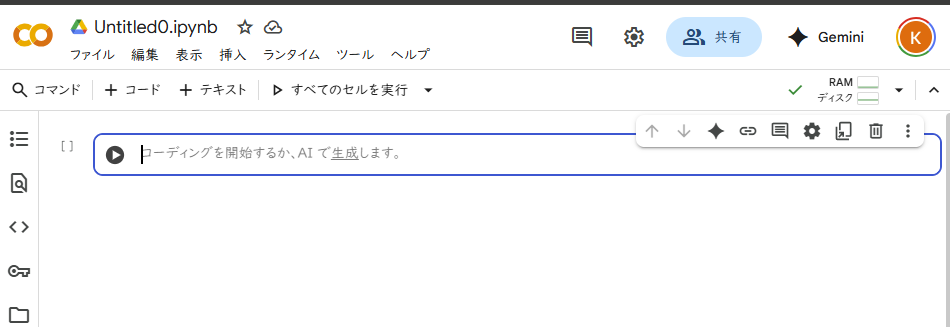
\includegraphics[width=11cm]{colab-notebook.png}};
      \end{scope}
      \draw[black!25,line width=.5pt] (.01,.01) rectangle (10.99,4.79);
      \draw[courseblue,line width=1pt,rounded corners=2mm,fill=black!2]
        (.25,2.4) rectangle (10.75,3.25);
      \fill[black!70] (.8,2.825) circle[radius=2.3mm];
      \fill[white] (.74,2.95) -- (.74,2.70) -- (.94,2.825) -- cycle;
      \node[anchor=west,font=\codefont\fontsize{20}{24}\selectfont]
        at (1.35,2.825) {\textcolor{codevalue}{1} + \textcolor{codevalue}{1}};
      \node[anchor=west,font=\codefont\fontsize{20}{24}\selectfont]
        at (1.35,1.55) {2};
      \node[anchor=west,text=courseblue] at (6.3,2.825)
        {\textbf{1}\quad セルに入力};
      \draw[courseblue,line width=1pt,-{Stealth[length=2mm]}]
        (6.1,2.825) -- (4.1,2.825);
      \node[anchor=west,text=courseblue] at (.3,.55)
        {\textbf{2}\quad \playicon で実行};
      \draw[courseblue,line width=1pt,-{Stealth[length=2mm]}]
        (.8,.9) -- (.8,2.46);
      \node[anchor=west,text=courseblue] at (6.3,1.55)
        {\textbf{3}\quad 結果を確認};
      \draw[courseblue,line width=1pt,-{Stealth[length=2mm]}]
        (6.1,1.55) -- (2.5,1.55);
      \node[anchor=south east,text=black!60,font=\fontsize{7}{9}\selectfont]
        at (10.75,.15) {セル部分は説明用に拡大・再現};
    \end{tikzpicture}
    \par}
  \vspace{1mm}
  {\small \playicon をクリックするか、\textbf{Ctrl+Enter}で実行します。\par}
  {\small 次の計算は、画面上部の\textbf{「＋コード」}でセルを追加します。\par}
\end{frame}

% 9 -------------------------------------------------------------------
\begin{frame}[t]{四則演算と累乗}
  \setlength{\parskip}{0pt}
  \begingroup\centering
    \renewcommand{\arraystretch}{1.0}
    \begin{tabular}{@{}>{\codefont}l@{\hspace{4mm}}l@{\hspace{4mm}}>{\codefont}l@{\hspace{4mm}}>{\codefont\color{codevalue}}r@{}}
      \multicolumn{1}{@{}l}{\textcolor{courseblue}{\textbf{演算子}}} &
      \textcolor{courseblue}{\textbf{意味}} &
      \multicolumn{1}{@{}l}{\textcolor{courseblue}{\textbf{計算例}}} &
      \multicolumn{1}{r@{}}{\textcolor{courseblue}{\textbf{結果}}} \\
      \hline
      +  & 足し算 & 7 + 2 & 9 \\
      -  & 引き算 & 7 - 2 & 5 \\
      *  & 掛け算 & 7 * 2 & 14 \\
      /  & 割り算（結果は小数） & 7 / 2 & 3.5 \\
      // & 割り算の商 & 7 // 2 & 3 \\
      \% & 割り算のあまり & 7 \% 2 & 1 \\
      ** & 累乗 & 2 ** 3 & 8
    \end{tabular}
    \par
  \endgroup
  \vspace{3mm}
  \setbeamercolor{arithmetic note}{fg=black,bg=courseblue!9}
  \begin{beamercolorbox}[wd=\textwidth,sep=1.8mm]{arithmetic note}
    \textbf{括弧の中を先に計算します。}\\[1mm]
    % Executable Python examples: keep * and show the output separately.
    {\codefont 2 + 3 * 4}\enspace →\enspace {\codefont\textcolor{codevalue}{14}}
    \hfill
    {\codefont (2 + 3) * 4}\enspace →\enspace {\codefont\textcolor{codevalue}{20}}
  \end{beamercolorbox}
  \par\vspace{2mm}
  {\small 好きな式を入力して、結果を確かめてみましょう。\par}
\end{frame}

% 10a: start with an executable example, then explain the name-value link.
\begin{frame}[t]{変数を使ってみよう}
  \setlength{\parskip}{0pt}
  新しいセルにスライドのコードを入力しましょう。
  \par\vspace{1mm}
  \setbeamercolor{example code}{fg=black,bg=black!4}
  \setbeamercolor{example output}{fg=black,bg=white}
  \begin{columns}[T,onlytextwidth]
    \begin{column}{.36\textwidth}
      \pythonexample{1}
        {a = \textcolor{codevalue}{5}}
        {a * \textcolor{codevalue}{2}}{10}
    \end{column}
    \begin{column}{.58\textwidth}
      \begingroup\centering
        \begin{tikzpicture}[x=1cm,y=1cm]
          \node[font=\small] at (.8,1.9) {変数名};
          \node[draw=courseblue,line width=1pt,rounded corners=2mm,
            minimum width=1.5cm,minimum height=1.2cm,
            text=courseblue,font=\codefont\fontsize{24}{28}\selectfont]
            (varname) at (.8,.9) {a};
          \node[font=\small] at (4.8,1.9) {値};
          \node[fill=courseblue!9,rounded corners=2mm,
            minimum width=1.5cm,minimum height=1.2cm,
            text=codevalue,font=\codefont\fontsize{24}{28}\selectfont]
            (varvalue) at (4.8,.9) {5};
          \draw[courseblue,line width=1.5pt,-{Stealth[length=3mm]}]
            (varname.east) -- (varvalue.west);
        \end{tikzpicture}\par
      \endgroup
      {\small {\codefont a * 2}は、\(5 \times 2 = 10\)の計算。\par}
    \end{column}
  \end{columns}
  \vspace{2mm}
  \textbf{変数は、値に付けて使う名前です。}
  \par
  \begin{itemize}
    \setlength{\itemsep}{1mm}
    \item 同じ値を繰り返し使える（{\codefont a + 3} → {\codefont 8}）
    \item 名前で意味を表せる（{\codefont length = 5}：長さ）
  \end{itemize}
  \vspace{1mm}
  \setbeamercolor{variable note}{fg=black,bg=courseblue!9}
  \begin{beamercolorbox}[wd=\textwidth,sep=1mm]{variable note}
    \small Pythonでは事前の変数宣言は不要です。\\
    {\codefont a = 5}のように、最初の代入で変数を定義します。
  \end{beamercolorbox}
\end{frame}

% 10b: execute in order and distinguish outputs from variable values.
\begin{frame}[t]{変数への代入と更新}
  \setlength{\parskip}{0pt}
  左から順に実行し、変数{\codefont a}の値を確かめましょう。
  \par\vspace{1mm}
  \setbeamercolor{example code}{fg=black,bg=black!4}
  \setbeamercolor{example output}{fg=black,bg=white}
  \setbeamercolor{assignment note}{fg=black,bg=courseblue!9}
  \begin{columns}[T,onlytextwidth]
    \begin{column}{.31\textwidth}
      \textcolor{courseblue}{\textbf{1\quad 定義と代入}}
      \pythonexample{1}
        {a = \textcolor{codevalue}{5}}
        {a * \textcolor{codevalue}{2}}{10}
      \par\vspace{1mm}
      {\small {\codefont a}の値：{\codefont\textcolor{codevalue}{5}}\par}
    \end{column}
    \begin{column}{.31\textwidth}
      \textcolor{courseblue}{\textbf{2\quad 値を変更}}
      \pythonexample{2}
        {a = \textcolor{codevalue}{8}}
        {a * \textcolor{codevalue}{2}}{16}
      \par\vspace{1mm}
      {\small {\codefont a}の値：{\codefont\textcolor{codevalue}{8}}\par}
    \end{column}
    \begin{column}{.31\textwidth}
      \textcolor{courseblue}{\textbf{3\quad 値を更新}}
      \pythonexample{3}
        {a = a + \textcolor{codevalue}{2}}
        {\textcolor{codebuiltin}{print}(a)}{10}
      \par\vspace{1mm}
      {\small {\codefont a}の値：{\codefont\textcolor{codevalue}{10}}\par}
    \end{column}
  \end{columns}
  \vspace{1mm}
  \begin{beamercolorbox}[wd=\textwidth,sep=1.5mm]{assignment note}
    \textbf{\texttt{=}は、右辺の値を左辺の変数に代入する記号です。}\\
    {\small 等号ではありません。{\codefont a = a + 2}は{\codefont a}を8から10へ更新します。\\
    {\codefont print(a)}は値の表示。セル末尾なら{\codefont a}だけでも表示できます。}
  \end{beamercolorbox}
\end{frame}

% 11a: compare values first, then name their types.
\begin{frame}[t]{型を調べてみよう}
  \setlength{\parskip}{0pt}
  {\codefont 5}・{\codefont 5.0}・{\codefont "5"}を、{\codefont type()}で比べてみましょう。
  \par\vspace{2mm}
  \setbeamercolor{example code}{fg=black,bg=black!4}
  \setbeamercolor{example output}{fg=black,bg=white}
  \begin{columns}[T,onlytextwidth]
    \begin{column}{.31\textwidth}
      \pythonexample{1}
        {a = \textcolor{codevalue}{5}}
        {\textcolor{codebuiltin}{type}(a)}{int}
      \par\vspace{1mm}
      {\small\textbf{整数型}\par}
    \end{column}
    \begin{column}{.31\textwidth}
      \pythonexample{2}
        {b = \textcolor{codevalue}{5.0}}
        {\textcolor{codebuiltin}{type}(b)}{float}
      \par\vspace{1mm}
      {\small\textbf{浮動小数点型}\par}
    \end{column}
    \begin{column}{.31\textwidth}
      \pythonexample{3}
        {c = \textcolor{codestring}{"5"}}
        {\textcolor{codebuiltin}{type}(c)}{str}
      \par\vspace{1mm}
      {\small\textbf{文字列型}\par}
    \end{column}
  \end{columns}
  \vspace{2mm}
  \textbf{型はデータの種類です。{\codefont type(値)}で調べます。}
  \par
  \begin{itemize}
    \setlength{\itemsep}{1mm}
    \item {\codefont float}は、小数を扱うための型です。
  \end{itemize}
  \vspace{1mm}
  \setbeamercolor{type note}{fg=black,bg=courseblue!9}
  \begin{beamercolorbox}[wd=\textwidth,sep=1.5mm]{type note}
    \small 引用符で囲むと文字列になります（{\codefont\textcolor{codestring}{"5"}}・{\codefont\textcolor{codestring}{'5'}}）。
  \end{beamercolorbox}
\end{frame}

% 11b: contrast int/float arithmetic, including true and floor division.
\begin{frame}[t]{整数と浮動小数点の演算}
  \setlength{\parskip}{0pt}
  \setbeamercolor{example code}{fg=black,bg=black!4}
  \setbeamercolor{example output}{fg=black,bg=white}
  \begin{columns}[T,onlytextwidth]
    \begin{column}{.31\textwidth}
      \pythonresult{1}
        {\textcolor{codevalue}{5} + \textcolor{codevalue}{2}}{7}
      \par
      {\small 結果の型：{\codefont int}\par}
    \end{column}
    \begin{column}{.31\textwidth}
      \pythonresult{2}
        {\textcolor{codevalue}{5.0} + \textcolor{codevalue}{2.0}}{7.0}
      \par
      {\small 結果の型：{\codefont float}\par}
    \end{column}
    \begin{column}{.31\textwidth}
      \pythonresult{3}
        {\textcolor{codevalue}{5} + \textcolor{codevalue}{2.0}}{7.0}
      \par
      {\small 結果の型：{\codefont float}\par}
    \end{column}
  \end{columns}
  \vspace{2mm}
  \textbf{加減乗算は、{\codefont float}を含むと結果も{\codefont float}です。}
  \par\vspace{1mm}
  \begingroup\centering
    \renewcommand{\arraystretch}{1.0}
    \begin{tabular}{@{}>{\codefont}l@{\hspace{5mm}}>{\codefont}l@{\hspace{5mm}}>{\codefont}l@{}}
      \multicolumn{1}{@{}l}{\textcolor{courseblue}{\textbf{演算}}} &
      \multicolumn{1}{@{}l}{\textcolor{courseblue}{\textbf{整数の入力}}} &
      \multicolumn{1}{@{}l@{}}{\textcolor{courseblue}{\textbf{小数を含む入力}}} \\
      \hline
      / & 5 / 2 → \textcolor{codevalue}{2.5} & 5.0 / 2 → \textcolor{codevalue}{2.5} \\
      // & 5 // 2 → \textcolor{codevalue}{2} & 5.0 // 2 → \textcolor{codevalue}{2.0}
    \end{tabular}\par
  \endgroup
  \vspace{1mm}
  \setbeamercolor{numeric note}{fg=black,bg=courseblue!9}
  \begin{beamercolorbox}[wd=\textwidth,sep=1mm]{numeric note}
    \small {\codefont /}は整数同士でも、結果が{\codefont float}になります。\\
    {\codefont //}は商を小さい側の整数値へ丸めます。
  \end{beamercolorbox}
\end{frame}

% 11c: Python int arithmetic is exact; floats have finite binary precision.
% Reference: https://docs.python.org/ja/3/tutorial/floatingpoint.html
\begin{frame}[t]{浮動小数点の計算と丸め誤差}
  \setlength{\parskip}{0pt}
  次の計算結果を確認してみましょう。
  \par\vspace{1mm}
  \setbeamercolor{example code}{fg=black,bg=black!4}
  \setbeamercolor{example output}{fg=black,bg=white}
  \pythonresult{1}
    {\textcolor{codevalue}{0.1} + \textcolor{codevalue}{0.2}}
    {0.30000000000000004}
  \par\vspace{1mm}
  \begin{itemize}
    \setlength{\itemsep}{2mm}
    \item Pythonの{\codefont int}：整数の加減乗算を正確に計算する
    \item {\codefont float}：有限桁の2進数で値を表す
      \begin{itemize}
        \item {\codefont 0.1}や{\codefont 0.2}は正確には表せず、近似する
        \item 値の表現や計算に、小さなずれが生じることがある
      \end{itemize}
  \end{itemize}
  \vspace{1mm}
  \setbeamercolor{rounding note}{fg=black,bg=courseblue!9}
  \begin{beamercolorbox}[wd=\textwidth,sep=1.5mm]{rounding note}
    \textbf{有限桁への丸めで生じるずれが、丸め誤差です。}
  \end{beamercolorbox}
  \par\vspace{1mm}
  {\small 浮動小数点の表現は、\textcolor{courseblue}{\textbf{11/24}}の授業で扱う予定です。\par}
\end{frame}

% 11d: connect the type distinction to arithmetic and conversions.
\begin{frame}[t]{型によって計算が変わる}
  \setlength{\parskip}{0pt}
  次の2つの計算結果を比べてみましょう。
  \par\vspace{1mm}
  \setbeamercolor{example code}{fg=black,bg=black!4}
  \setbeamercolor{example output}{fg=black,bg=white}
  \begin{columns}[T,onlytextwidth]
    \begin{column}{.48\textwidth}
      \pythonresult{1}
        {\textcolor{codevalue}{5} + \textcolor{codevalue}{2}}{7}
    \end{column}
    \begin{column}{.48\textwidth}
      \pythonresult{2}
        {\textcolor{codestring}{"5"} + \textcolor{codestring}{"2"}}
        {\textcolor{codestring}{'52'}}
    \end{column}
  \end{columns}
  \vspace{2mm}
  \textbf{数値の{\codefont +}は足し算、文字列の{\codefont +}は連結です。}
  \par\vspace{1mm}
  {\codefont "5" + 2}はエラーになります。\\
  文字列を数値に変換してから、計算しましょう。
  \par\vspace{2mm}
  \begingroup\centering
    \renewcommand{\arraystretch}{1.0}
    \begin{tabular}{@{}l@{\hspace{5mm}}>{\codefont}l@{\hspace{5mm}}>{\codefont\color{codevalue}}r@{}}
      \textcolor{courseblue}{\textbf{変換}} &
      \multicolumn{1}{@{}l}{\textcolor{courseblue}{\textbf{計算例}}} &
      \multicolumn{1}{r@{}}{\textcolor{courseblue}{\textbf{結果}}} \\
      \hline
      整数に変換 & \textcolor{codebuiltin}{int}(\textcolor{codestring}{"5"}) + 2 & 7 \\
      小数に変換 & \textcolor{codebuiltin}{float}(\textcolor{codestring}{"5"}) + 2 & 7.0
    \end{tabular}\par
  \endgroup
\end{frame}

% 11e: import NumPy, then call a function using its short name.
% References: https://numpy.org/doc/stable/user/absolute_beginners.html
% https://numpy.org/doc/stable/reference/routines.math.html
\begin{frame}[t]{NumPyを使ってみよう}
  \setlength{\parskip}{0pt}
  まず、平方根$\sqrt{9}$を計算してみましょう。
  \par\vspace{1mm}
  \setbeamercolor{example code}{fg=black,bg=black!4}
  \setbeamercolor{example output}{fg=black,bg=white}
  \pythonexample{1}
    {\textcolor{codebuiltin}{import} numpy \textcolor{codebuiltin}{as} np}
    {\textcolor{codebuiltin}{print}(np.\textcolor{codebuiltin}{sqrt}(\textcolor{codevalue}{9}))}{3.0}
  \par\vspace{1mm}
  \begin{itemize}
    \setlength{\itemsep}{1mm}
    \item NumPyは、数値計算の道具を集めたライブラリです。
    \item {\codefont import}で読み込み、{\codefont as np}で短い名前を付けます。
    \item 内側の{\codefont np.sqrt(9)}で計算 → 外側の{\codefont print()}で表示
  \end{itemize}
  \vspace{1mm}
  \setbeamercolor{numpy note}{fg=black,bg=courseblue!9}
  \begin{beamercolorbox}[wd=\textwidth,sep=1.2mm]{numpy note}
    \small 円周率$\pi$は{\codefont np.pi}、自然対数の底$e$は{\codefont np.e}です。\\
    Colabを再起動したら、読み込みのセルをもう一度実行します。
  \end{beamercolorbox}
\end{frame}

% 11f: connect a familiar angle to radians and degree conversion.
% Reference: https://numpy.org/doc/stable/reference/generated/numpy.sin.html
\begin{frame}[t]{三角関数を計算しよう}
  \setlength{\parskip}{0pt}
  \setbeamercolor{example code}{fg=black,bg=black!4}
  \setbeamercolor{example output}{fg=black,bg=white}
  \pythonresult{2}
    {\textcolor{codebuiltin}{print}(np.\textcolor{codebuiltin}{sin}(np.pi / \textcolor{codevalue}{2}))}{1.0}
  \par\vspace{2mm}
  \begin{columns}[T,onlytextwidth]
    \begin{column}{.31\textwidth}
      \centering $\sin x$（正弦）\par
      {\codefont np.\textcolor{codebuiltin}{sin}(x)}
    \end{column}
    \begin{column}{.31\textwidth}
      \centering $\cos x$（余弦）\par
      {\codefont np.\textcolor{codebuiltin}{cos}(x)}
    \end{column}
    \begin{column}{.31\textwidth}
      \centering $\tan x$（正接）\par
      {\codefont np.\textcolor{codebuiltin}{tan}(x)}
    \end{column}
  \end{columns}
  \vspace{2mm}
  \setbeamercolor{angle note}{fg=black,bg=courseblue!9}
  \begin{beamercolorbox}[wd=\textwidth,sep=1.5mm]{angle note}
    \textbf{角度の単位はラジアンです。}\quad $\pi\,\mathrm{rad}=180^\circ$\\[1mm]
    \small 度から変換するときは{\codefont np.deg2rad()}を使います。\\
    $\sin 30^\circ$：{\codefont np.sin(np.deg2rad(30))}\enspace → 約0.5
  \end{beamercolorbox}
  \par\vspace{1mm}
  {\small {\codefont np.sin(30)}は「30ラジアン」の計算になります。\par}
\end{frame}

% 11g: distinguish the logarithm bases and the exponential function.
% Reference: https://numpy.org/doc/stable/reference/generated/numpy.log.html
\begin{frame}[t]{指数関数と対数関数}
  \setlength{\parskip}{0pt}
  \setbeamercolor{example code}{fg=black,bg=black!4}
  \setbeamercolor{example output}{fg=black,bg=white}
  \begin{columns}[c,onlytextwidth]
    \begin{column}{.65\textwidth}
      \pythonresult{3}
        {\textcolor{codebuiltin}{print}(np.\textcolor{codebuiltin}{log10}(\textcolor{codevalue}{1000}))}{3.0}
    \end{column}
    \begin{column}{.30\textwidth}
      \centering $10^3=1000$\par
      なので\par
      $\log_{10}1000=3$
    \end{column}
  \end{columns}
  \par\vspace{2mm}
  \begingroup\centering
    \renewcommand{\arraystretch}{1.05}
    \begin{tabular}{@{}l@{\hspace{5mm}}>{\codefont}l@{\hspace{5mm}}>{\codefont}l@{}}
      \textcolor{courseblue}{\textbf{数学での表記}} &
      \multicolumn{1}{l}{\textcolor{courseblue}{\textbf{書き方}}} &
      \multicolumn{1}{l@{}}{\textcolor{courseblue}{\textbf{計算例 → 結果}}} \\
      \hline
      $e^x$ & np.\textcolor{codebuiltin}{exp}(x) & np.exp(0) → \textcolor{codevalue}{1.0} \\
      $\ln x=\log_e x$ & np.\textcolor{codebuiltin}{log}(x) & np.log(np.e) → \textcolor{codevalue}{1.0} \\
      $\log_{10}x$ & np.\textcolor{codebuiltin}{log10}(x) & np.log10(100) → \textcolor{codevalue}{2.0} \\
      $\log_2 x$ & np.\textcolor{codebuiltin}{log2}(x) & np.log2(8) → \textcolor{codevalue}{3.0}
    \end{tabular}\par
  \endgroup
  \vspace{2mm}
  \setbeamercolor{log note}{fg=black,bg=courseblue!9}
  \begin{beamercolorbox}[wd=\textwidth,sep=1.5mm]{log note}
    \textbf{\codefont np.log}\textbf{は、底が$e$の自然対数です。}\\
    \small 実数の範囲では、対数の入力は正の値にします。
  \end{beamercolorbox}
\end{frame}

% 11h: a first taste of arrays and evenly spaced sample points.
\begin{frame}[t]{配列でまとめて計算しよう}
  \setlength{\parskip}{0pt}
  \setbeamercolor{example code}{fg=black,bg=black!4}
  \setbeamercolor{example output}{fg=black,bg=white}
  \pythonexample{4}
    {x = np.\textcolor{codebuiltin}{array}([\textcolor{codevalue}{1}, \textcolor{codevalue}{4}, \textcolor{codevalue}{9}])}
    {\textcolor{codebuiltin}{print}(np.\textcolor{codebuiltin}{sqrt}(x))}{[1. 2. 3.]}
  \par\vspace{1mm}
  \textbf{配列は、複数の値をまとめて扱うためのものです。}
  \par
  \begin{itemize}
    \setlength{\itemsep}{1mm}
    \item {\codefont np.array([1, 4, 9])}で、3個の値をまとめます。
    \item {\codefont np.sqrt(x)}は、各要素の平方根を計算します。
  \end{itemize}
  \vspace{1mm}
  \setbeamercolor{array note}{fg=black,bg=courseblue!9}
  \begin{beamercolorbox}[wd=\textwidth,sep=1.5mm]{array note}
    \small {\codefont x * 2}なら、各要素を2倍して{\codefont [2 8 18]}になります。\\
    {\codefont np.sin(x)}や{\codefont np.log(x)}でも、まとめて計算できます。
  \end{beamercolorbox}
\end{frame}

% 11i: visualize the start, end, and number of sample points.
\begin{frame}[t]{等間隔の値を作ろう}
  \setlength{\parskip}{0pt}
  \setbeamercolor{example code}{fg=black,bg=black!4}
  \setbeamercolor{example output}{fg=black,bg=white}
  \pythonexample{5}
    {x = np.\textcolor{codebuiltin}{linspace}(\textcolor{codevalue}{0}, \textcolor{codevalue}{1}, \textcolor{codevalue}{5})}
    {\textcolor{codebuiltin}{print}(x)}{[0.\enspace 0.25\enspace 0.5\enspace 0.75\enspace 1.]}
  \par\vspace{2mm}
  \begingroup\centering
    \begin{tikzpicture}[x=1cm,y=1cm]
      \draw[courseblue,line width=1pt] (0,0) -- (8.8,0);
      \foreach \pos/\val in {0/0,2.2/0.25,4.4/0.5,6.6/0.75,8.8/1}{
        \fill[courseblue] (\pos,0) circle[radius=1.5mm];
        \node[below=2mm,font=\small] at (\pos,0) {\(\val\)};
      }
      \node[above=2mm,font=\small] at (0,0) {開始};
      \node[above=2mm,font=\small] at (8.8,0) {終了};
    \end{tikzpicture}\par
  \endgroup
  \vspace{2mm}
  \setbeamercolor{spacing note}{fg=black,bg=courseblue!9}
  \begin{beamercolorbox}[wd=\textwidth,sep=1.2mm]{spacing note}
    {\codefont np.linspace(開始, 終了, 個数)}\\
    \small 両端を含む、指定した個数の値を作ります。
  \end{beamercolorbox}
  \par
  \vspace{1mm}
  {\small 配列の詳しい使い方は、\textcolor{courseblue}{\textbf{11/10}}の授業で扱います。\par}
\end{frame}

% 11j: combine functions and arithmetic in one executable expression.
\begin{frame}[t]{数式をコードにしてみよう}
  \setlength{\parskip}{0pt}
  \(y=e^{-x}\sin x\)を、\(x=\dfrac{\pi}{2}\)で計算してみましょう。
  \par\vspace{1mm}
  \setbeamercolor{example code}{fg=black,bg=black!4}
  \setbeamercolor{example output}{fg=black,bg=white}
  \begin{beamercolorbox}[wd=\textwidth,sep=1.8mm]{example code}
    {\codefont\fontsize{9}{10}\selectfont\textcolor{courseblue}{In [6]:}\par}
    \begingroup\codefont\fontsize{16}{18}\selectfont
      x = np.pi / \textcolor{codevalue}{2}\\
      y = np.\textcolor{codebuiltin}{exp}(-x) * np.\textcolor{codebuiltin}{sin}(x)\\
      \textcolor{codebuiltin}{print}(y)\par
    \endgroup
  \end{beamercolorbox}\par
  \begin{beamercolorbox}[wd=\textwidth,sep=.5mm,leftskip=1.3mm]{example output}
    {\fontsize{9}{11}\selectfont\textcolor{black!65}{出力}}\quad
    {\codefont\fontsize{16}{18}\selectfont 0.20787957635076193}
  \end{beamercolorbox}
  \par\vspace{1mm}
  \begin{itemize}
    \setlength{\itemsep}{1mm}
    \item 掛け算は{\codefont *}で書き、{\codefont x}を変えたら計算し直します。
  \end{itemize}
  \vspace{1mm}
  \setbeamercolor{combine note}{fg=black,bg=courseblue!9}
  \begin{beamercolorbox}[wd=\textwidth,sep=1.5mm]{combine note}
    \small {\codefont x = np.linspace(0, 2 * np.pi, 9)}に変えてみましょう。\\
    配列なら、同じ式で各要素の$y$をまとめて計算できます。\\[1mm]
    表示例：{\codefont 3.2e-01}\enspace $=3.2\times10^{-1}=0.32$
  \end{beamercolorbox}
\end{frame}

% 12 ------------------------------------------------------------------
\begin{frame}[t]{ノートブックのダウンロード}
  \setlength{\parskip}{0pt}
  Colabのメニューを、次の順に選びます。
  \par\vspace{2mm}
  \begingroup\centering
    \begin{tikzpicture}[x=1cm,y=1cm]
      \path[use as bounding box] (0,-.05) rectangle (10.7,3.65);
      \foreach \y/\num in {3/1,1.7/2,.4/3}{
        \fill[courseblue!7,rounded corners=1.5mm]
          (.9,\y-.48) rectangle (10.7,\y+.48);
        \node[circle,fill=courseblue,text=white,inner sep=0,
          minimum size=7mm,font=\bfseries\fontsize{14}{16}\selectfont]
          at (.35,\y) {\num};
      }
      \foreach \top/\bottom in {2.56/2.16,1.26/.86}{
        \draw[courseblue,line width=1.2pt,-{Stealth[length=2mm]}]
          (.35,\top) -- (.35,\bottom);
      }
      \node[anchor=west,font=\bfseries\fontsize{14}{17}\selectfont]
        at (1.1,3) {ファイル};
      \node[anchor=west,font=\small,text=black!70]
        at (6.6,3) {画面左上のメニュー};
      \node[anchor=west,font=\bfseries\fontsize{14}{17}\selectfont]
        at (1.1,1.7) {ダウンロード};
      \node[anchor=west,font=\small,text=black!70]
        at (6.6,1.7) {保存形式を表示する};
      \node[anchor=west,font=\bfseries\fontsize{14}{17}\selectfont]
        at (1.1,.4) {.ipynb をダウンロード};
      \node[anchor=west,font=\small,text=black!70]
        at (6.6,.4) {PCに保存する};
    \end{tikzpicture}\par
  \endgroup
  \vspace{3mm}
  \setbeamercolor{submission note}{fg=black,bg=courseblue!9}
  \begin{beamercolorbox}[wd=\textwidth,sep=2mm]{submission note}
    \textbf{提出対象は、授業で用いたノートブックです。}\\[1mm]
    \small 保存した\textcolor{courseblue}{.ipynb}ファイルを、\\
    学務情報システムにアップロードしてください。
  \end{beamercolorbox}
\end{frame}

% 13 ------------------------------------------------------------------
\begin{frame}[t]{講義資料のダウンロード}
  \setlength{\parskip}{0pt}
  授業で使うコードは、GitHubから入手します。\\
  {\small\url{https://github.com/nogaki/Computational_Physics_B}\par}
  \vspace{2mm}
  \begingroup\centering
    \begin{tikzpicture}[x=1cm,y=1cm]
      \path[use as bounding box] (0,-.05) rectangle (10.7,3.4);
      \foreach \y/\num in {2.8/1,1.65/2,.5/3}{
        \fill[courseblue!7,rounded corners=1.5mm]
          (.9,\y-.43) rectangle (10.7,\y+.43);
        \node[circle,fill=courseblue,text=white,inner sep=0,
          minimum size=7mm,font=\bfseries\fontsize{14}{16}\selectfont]
          at (.35,\y) {\num};
      }
      \foreach \top/\bottom in {2.36/2.11,1.21/.96}{
        \draw[courseblue,line width=1.2pt,-{Stealth[length=2mm]}]
          (.35,\top) -- (.35,\bottom);
      }
      \node[anchor=west,font=\bfseries\fontsize{14}{17}\selectfont]
        at (1.1,2.8) {講義のフォルダーを開く};
      \node[anchor=west,font=\small,text=black!70]
        at (7.1,2.8) {例：{\codefont 2026/week1}};
      \node[anchor=west,font=\bfseries\fontsize{14}{17}\selectfont]
        at (1.1,1.65) {ノートブックを開く};
      \node[anchor=west,font=\small,text=black!70]
        at (7.1,1.65) {{\codefont week1.ipynb}};
      \node[anchor=west,font=\bfseries\fontsize{14}{17}\selectfont]
        at (1.1,.5) {ダウンロードする};
      % Editable enlarged download button, based on the source GitHub screenshot.
      \draw[courseblue,fill=white,line width=.8pt,rounded corners=1.2mm]
        (5.8,.12) rectangle (6.56,.88);
      \draw[courseblue,line width=1.6pt,line cap=round,line join=round]
        (6.18,.75) -- (6.18,.38)
        (6.02,.54) -- (6.18,.38) -- (6.34,.54)
        (5.93,.37) -- (5.93,.25) -- (6.43,.25) -- (6.43,.37);
      \node[anchor=west,font=\small,text=black!70]
        at (6.7,.5) {ファイル表示の右上};
    \end{tikzpicture}\par
  \endgroup
  \vspace{1mm}
  \setbeamercolor{materials note}{fg=black,bg=courseblue!9}
  \begin{beamercolorbox}[wd=\textwidth,sep=1.5mm]{materials note}
    \textbf{授業前にダウンロードし、Colabで開きましょう。}\\[1mm]
    \small 「ノートブックを開く」→「アップロード」で、\\
    保存した{\codefont week1.ipynb}を選びます。
  \end{beamercolorbox}
\end{frame}

% 14 ------------------------------------------------------------------
\begin{frame}[t]{実習タイム}
  \setlength{\parskip}{0pt}
  \textbf{超高性能電卓として遊んでみよう！}
  \par\vspace{2mm}
  \begin{itemize}
    \setlength{\itemsep}{3mm}
    \item 三角関数の値を比べる
      \begin{itemize}
        \item 角度を$0^\circ$、$30^\circ$、$60^\circ$、$90^\circ$に変え、$\sin$と$\cos$を計算。
        \item ヒント：{\codefont np.deg2rad()}でラジアンに変換。
      \end{itemize}
    \item 指数関数と対数関数の関係を確かめる
      \begin{itemize}
        \item {\codefont x}を$-2$・$0$・$2$に変え、{\codefont np.log(np.exp(x))}を計算。
      \end{itemize}
    \item $\sin^2 x+\cos^2 x=1$を確かめる
      \begin{itemize}
        \item {\codefont np.sin(x)**2 + np.cos(x)**2}を、好きな{\codefont x}で計算。
      \end{itemize}
  \end{itemize}
  \vspace{2mm}
  \setbeamercolor{practice note}{fg=black,bg=courseblue!9}
  \begin{beamercolorbox}[wd=\textwidth,sep=1.5mm]{practice note}
    \small 予想してから実行しましょう。{\codefont e-17}は$\times10^{-17}$の意味です。\\
    理論値との小さなずれが出たら、丸め誤差も思い出してください。
  \end{beamercolorbox}
\end{frame}

\end{document}
